\documentclass[11pt]{article}
%\usepackage{geometry}              % See geometry.pdf to learn the layout options. There are lots.

\usepackage[margin=1in]{geometry}
\geometry{letterpaper}                   % ... or a4paper or a5paper or ... 
%\geometry{landscape}                % Activate for for rotated page geometry
%\usepackage[parfill]{parskip}    % Activate to begin paragraphs with an empty line rather than an indent
\usepackage{graphicx}
\usepackage{amssymb}
\usepackage{epstopdf}
\usepackage{subfigure}
\usepackage{fancyvrb}
\usepackage{tabularx}
\usepackage{framed}
\usepackage{float}

\usepackage{graphicx,amsmath,amsthm,url,color,amsfonts}
\DeclareMathOperator*{\argmax}{arg\,max}
\DeclareMathOperator*{\argmin}{arg\,min}
\newcommand{\abs}[1]{ \left| #1 \right|} 

\usepackage{graphicx,amsmath,amsthm,url,color}
\usepackage{subfigure}

\usepackage[verbose]{wrapfig}
\usepackage{setspace,colortbl}
\usepackage{verbatim}


%%This is how we will set up code w/in the Text.
%\begin{Verbatim}[frame=single]
%stuff
%\end{Verbatim}


\DeclareGraphicsRule{.tif}{png}{.png}{`convert #1 `dirname #1`/`basename #1 .tif`.png}

\title{User Guide for GASV and GASVPro (Version 2.0)}
%\author{The Author}
\date{}                                           % Activate to display a given date or no date

\begin{document}
\maketitle

\tableofcontents
\clearpage

\section{Introduction}

GASV is software to identify structural variants from paired-end mapping data. \\

\noindent If you use GASV in your research, please cite: \\ \\
S. Sindi, E. Helman, A. Bashir, B.J. Raphael. A Geometric Approach for
Classification and Comparison of Structural Variants. Joint: 17th
Annual International Conference on Intelligent Systems in Molecular
Biology and 8th Annual International European Conference on
Computational Biology (ISMB/ECCB 09).  Bioinformatics 2009
25(12):i222-i230.\\

\noindent This product includes software developed by the Solution Engineering,
Inc. (http://www.seisw.com/). \\

\noindent Contact: Benjamin Raphael at gasv@cs.brown.edu \\

\noindent Version: 2.0 \\
\noindent Version Date: May 30 2012

\begin{wrapfigure}{r}{0.5\textwidth}
  \begin{center}
    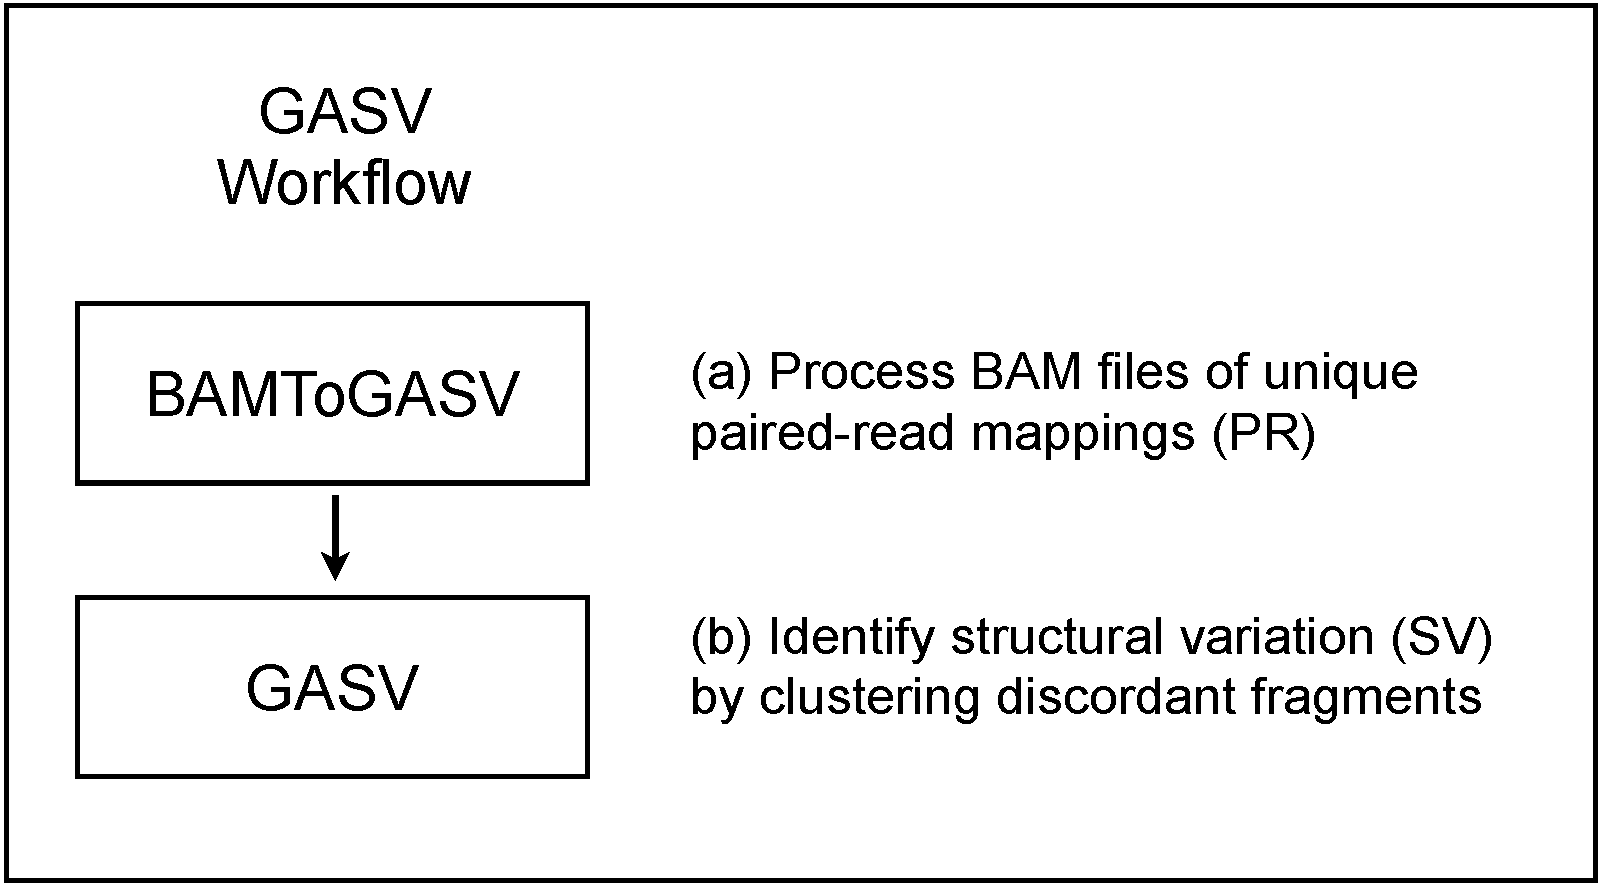
\includegraphics[width=0.5\textwidth]{Figures/GASV_Workflow.pdf}
  \end{center}
  \caption{\textbf{GASV Workflow}}
  \label{fig:GASVWorkflow}
\end{wrapfigure}


\subsection{Summary}

The GASV software utilizes a geometric algorithm to predict structural variation (SV) from a set of discordant mappings of paired-reads (PRs). 

\subsection{Requirements}
Requires: Perl, Java 5 (or higher), *nix OS, \\
\noindent Tested with: Perl v5.10.0, Java 6, Linux 2.6.26 \\

\noindent Building GASV from the source requires ant, available at: 
http://ant.apache.org/


\subsection{GASV Workflow}

The primary GASV workflow is an analysis pipeline for SV detection from a set of paired-end mappings (PEM) given in the form of a BAM file. In most workflows the BAM file is pre-processed for analysis with GASV using BAMToGASV (Figure~\ref{fig:GASVWorkflow}(a)) followed by analysis with GASV (Figure~\ref{fig:GASVWorkflow}(b)) to determine a set of potential SVs genome wide. Further downstream analysis of GASV predictions may be conducted with GASVPro, a probabilistic algorithm which integrates read-depth (RD) to improve specificity by eliminating false-positive predictions. 

\subsection{GASV Algorithm}
The GASV algorithm reports structural variant events defined by clusters of discordantly mapped fragments and explicitly represents uncertainty variant endpoints. We briefly overview the approach used in GASV; for a more detailed discussion of the GASV algorithm, refer to Sindi et al. (2009).

\begin{wrapfigure}{l}{0.5 \textwidth}
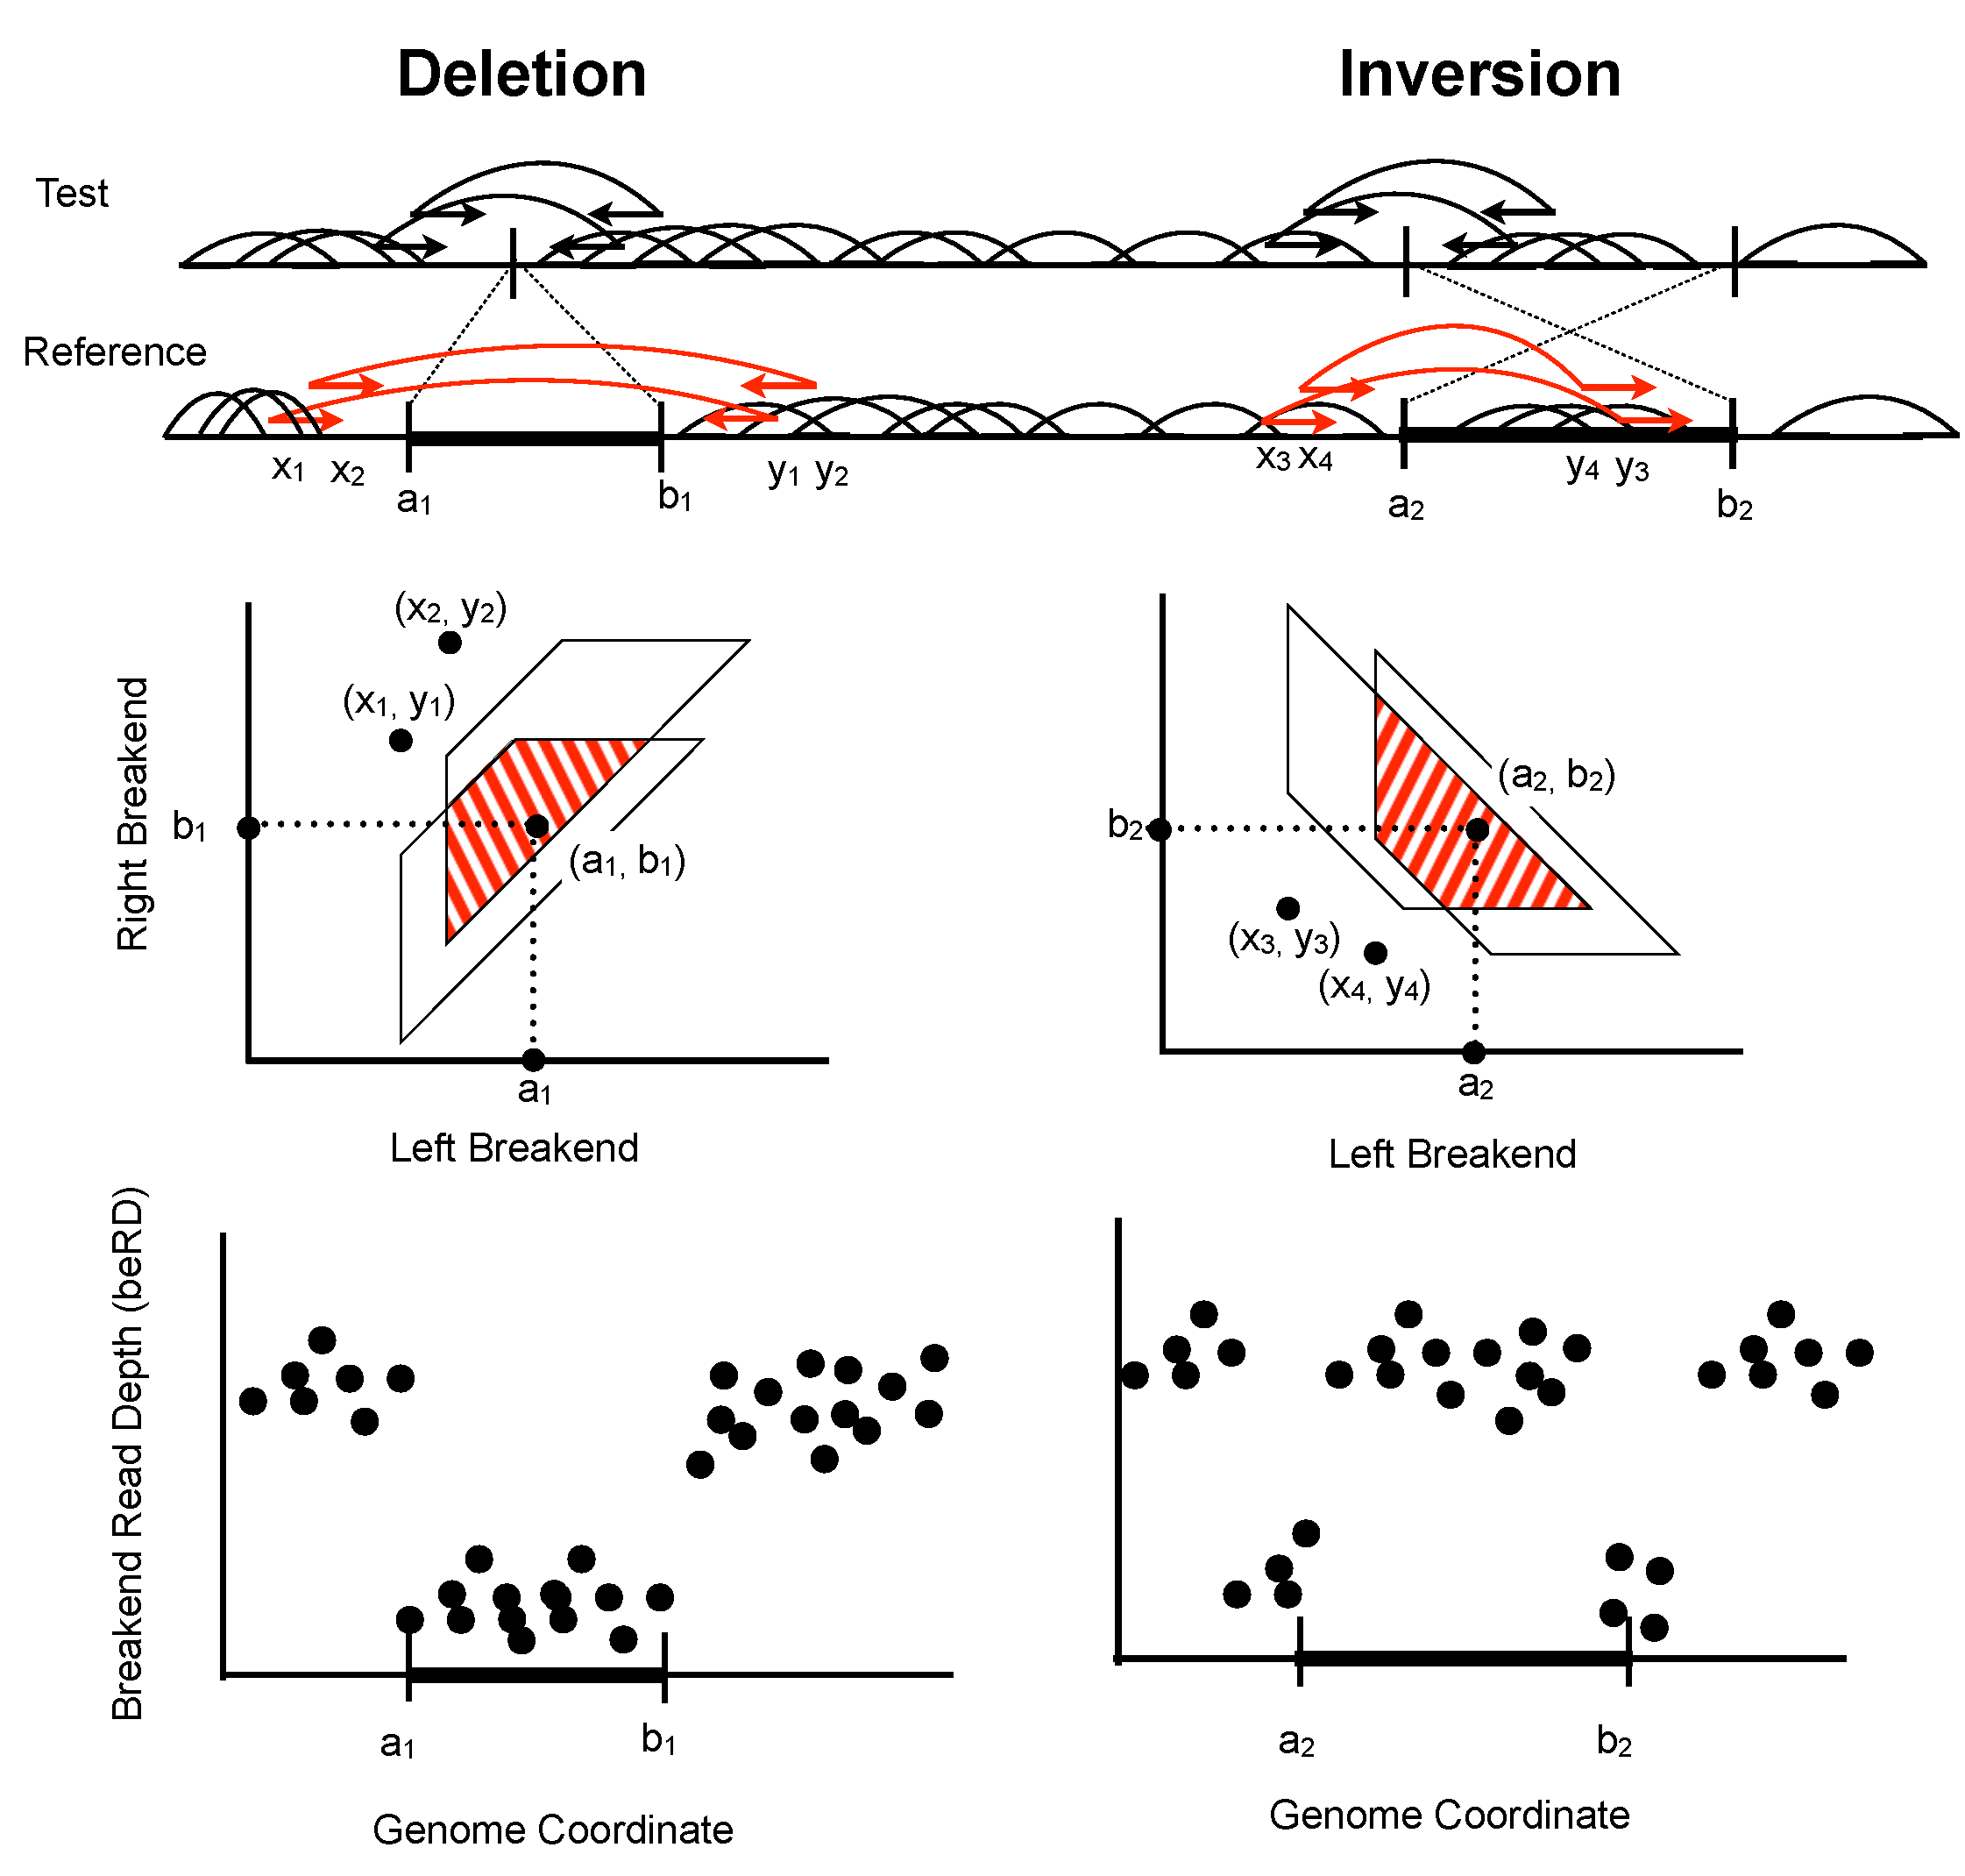
\includegraphics[width = 0.5 \textwidth] {Figures/GASV_Illustration.pdf} % requires the graphicx package
\caption{\textbf{GASV Algorithm of Structural Variation Detection from Paired-End Sequencing.}  (Top) Fragments (black arches) from a test genome are sequenced from both ends and the resulting paired reads are mapped to a reference genome. Fragments containing the breakpoint of a structural variant (black arches with arrows) have a discordant mapping (red).  (Bottom) GASV represents the uncertainty in breakpoint location as a breakend polygon (black trapezoids). GASV clusters fragments by computing polygon intersections (shaded red trapezoid) which correspond to fragments supporting the same variant.}
   \label{fig:illustration}
\end{wrapfigure}

A discordant mapping indicates a structural variant in the test genome defined by a novel adjacency $(a,b)$, where positions $a$ and $b$ are adjacent in the test genome, but not in the reference genome (see Figure~\ref{fig:illustration}). A single fragment alone does not uniquely specify the pair of breakends $(a,b)$ defining the rearrangement, but rather defines uncertainty in the location of the breakends. Formally, if we assume that a discordant fragment corresponds to exactly one structural variant, then the mapped locations, $x$ and $y$, of the fragment endpoints (without loss of generality we restrict $x < y$), and the breakends $a$ and $b$ satisfy
\begin{equation}
L_{\min} \le \text{sign}(x)(a - x) + \text{sign}(y) (b - y) \le L_{\max}, \nonumber
\label{eqn:trap}
\end{equation}
\noindent where sign$(x)$ and sign$(y)$ are $1$ if the reads align to the positive strand and have convergent orientation and $-1$ otherwise. Here we assume convergent orientation is when reads have opposite orientation with the left read forward and the right read reversed as in the case for Illumina sequencing technology. (Other sequencing protocols will may have different notions of convergent orientation.)  The inequality~(\ref{eqn:trap}) defines a trapezoid in the plane; discordant fragments corresponding to the same structural variant will have overlapping trapezoids and their intersection can be used to further refine the uncertainty in breakend location as in Figure~\ref{fig:illustration}. The final set of SV predictions from GASV corresponds to these polygonal intersections. 

\subsection{Installation}

You may either download executable jar files from\\

\noindent http://code.google.com/p/gasv/downloads/ \\

\noindent or build our code directly from the source.  

Building GASV from the source requires ant, available at: http://ant.apache.org/. To install from the source check out a read-only working copy from 

\begin{framed}
{\normalsize
\noindent \texttt{\% svn checkout http://gasv.googlecode.com/svn/trunk/ gasv-read-only}
}
\end{framed}

\noindent and install from the command line with ant

\begin{framed}
{\normalsize
\noindent \texttt{\% ant}
}
\end{framed}

\noindent During installation the java *class files are built into the build subdirectory. After installation the following executable jar files are created:
	
\begin{framed}
{\normalsize
\noindent \texttt{bin/GASV.jar }\\
\noindent \texttt{bin/BAMToGASV.jar }
}
\end{framed}

\section{Quickstart Guide to GASV}

This Quickstart Guide will demonstrate many features of GASV including determining the 
structural variants from paired-read sequences (PRs) whose mappings 
are encoded in a BAM file.

To demonstrate using BAMToGASV preprocessor in conjunction with GASV, we will use the file ``Example.bam'' available as a separate download from the GASV website:

\begin{framed}
\begin{Verbatim}
http://code.google.com/p/gasv
\end{Verbatim}
\end{framed}

More documentation is available for both GASV and BAMToGASV Preprocessor 
in sections below.  

\subsection{Using BAMToGASV to Preprocess BAM files}

The following command creates GASV input files by considering paired-reads (PRs) 
from the BAM file ``Example.bam" (this particular BAM file contains no library information and contains only reads from chr17, so no translocations):
\begin{framed}
{\normalsize
\begin{Verbatim}
% java -Xms512m -Xmx2048m -jar BAMToGASV.jar Example.bam
\end{Verbatim}
}
\end{framed}

As we detail further below, there are many options available for BAMToGASV. For example, use a minimum quality of $30$ and determine Lmin/Lmax by 3 standard deviations away from the mean, the command is

\begin{framed}
{\scriptsize
\begin{Verbatim}
% java -Xms512m -Xmx2048m -jar BAMToGASV.jar Example.bam -MAPPING_QUALITY 30 -CUTOFF_LMINLMAX SD=3
\end{Verbatim}
}
\end{framed}

If the BAM file contains multiple libraries, to process them as one set (rather than indvididually) the command is
\begin{framed}
{\small
\begin{Verbatim}
% java -Xms512m -Xmx2048m -jar BAMToGASV.jar Example.bam -LIBRARY_SEPARATED all
\end{Verbatim}
}
\end{framed}

\noindent Running the above command creates the following files:\\

\noindent Example.bam.info\\
\noindent Example.bam.gasv.in \\
\noindent Example.bam\_all.deletion \\
\noindent Example.bam\_all.divergent \\
\noindent Example.bam\_all.insertion \\
\noindent Example.bam\_all.inversion \\
\noindent Example.bam\_all.translocation\\

Example.info contains information about the concordant fragment length
distribution.   Example.gasv.in is a batch file of all PR files (except insertions) for input to the GASV program.
The rest of the files are PR files in the GASV input format, separated by variant type.

\subsection{Run GASV to Compute Structural Variants}

The following command will report inversion, deletion and divergent structural variants using the batch input file produced by BAMToGASV. Note the default behavior of GASV is to only report variants with at least 4 supporting fragments.  
In addition, if GASV.jar has not been added to the PATH, then a fully qualified pathname must be used.

\begin{framed}
{\small
\begin{Verbatim}
% java -jar GASV.jar --batch Example.bam.gasv.in
\end{Verbatim}
}
\end{framed}

Below is the contents of the *clusters file created, Example.bam.gasv.in.clusters:

\begin{framed}
{ \scriptsize
\begin{Verbatim}
#Cluster_ID: LeftChr: LeftBreakPoint:    RightChr: RightBreakPoint:   Num PRS: Localization: Type:
c99          17       660077,660155      17        660177,660255      4        39.8          D
c106         17       685625,685815      17        685996,686186      4        100.6         D
c4552        17       34908617,34908798  17        34908870,34909051  5        68.4          D
c5262        17       40566182,40566317  17        40567335,40567462  4        68.3          IR
c6367        17       50617507,50617679  17        50617548,50617720  4        87.8          D
\end{Verbatim}
}
\end{framed}
The tab separated fields indicate that there are 5 predictions, 4 deletions and 1 
inversion structural variant on chromosome 17. Examining the fourth line more carefully, cluster c5262 supports an inversion with left breakpoint occurs between positions 40566182, 40566316 and the 
right breakpoint between positions 40567335, 40567462.

In addition, the final columns tell us:
\begin{itemize}
\item 4 fragments support this SV (Num PRs = 4)
\item The breakpoint localization is 68. 
		The smaller the localization the more precisely the
		structural variant breakpoint is determined. Refer below and to Sindi, et al. (2009)  for more discussion 
		of localization.
\item This variant is a reciprocal inversion (Type = IR)
		Among the 4 PRs at least one is in the ++ orientation 
		(contains the left breakpoint) and one in the 
		-{}- orientation (contains the right breakpoint). 
\end{itemize}

\subsection{Useful GASV Examples} 
\begin{enumerate}

\item -{}-minClusterSize $<$val$>$
Report only predictions with at least a minimum number of supporting 
fragments. (By default, this parameter is set to 4.) For increased sensitivity, users can lower the threshold. For example to obtain all predictions supported by at least 2 mappings:

\begin{framed}
{ \small
\begin{Verbatim}
% java -jar GASV.jar --minClusterSize 2 --batch Example.bam.gasv.in
\end{Verbatim}
}
\end{framed}

\item -{}-maximal
In some cases a set of overlapping fragments may correspond to 
multiple breakpoints. The ``-{}-maximal" option will output 
all maximal breakpoint events.

\item -{}-maxPairedEndsPerWin $<$val$>$
The speed at which GASV runs corresponds to the number of fragments in 
a particular genomic region. Often some genomic regions (such as centromeres) 
will have a high density of discordant fragments. GASV's running time
can be significantly increased by skipping such high density regions with 
the ``-{}-maxPairedEndsPerWin'' option.

\item -{}-output $<$val$>$
As we detail below, there are three different output formats
that can be specified for *clusters file. The reads format, ``-{}-output reads'' 
will list the names of the reads in a cluster. 

\begin{framed}
{\small
\begin{Verbatim}
% java -jar GASV.jar --output reads --batch Example.bam.gasv.in
\end{Verbatim}
}
\end{framed}

\end{enumerate}

\clearpage
\section{BAMToGASV}

BAMToGASV generates GASV formatted input files from the SAM/BAM alignment format. SAM files are also accepted as input, but for clarity this manual will refer to BAM files only.  Picard, a Java tool for processing BAM files, is packaged in the JAR file. Running BAMToGASV with no arguments produces basic usage information.

\subsection{Requirements}
   
BAMToGASV is currently designed to process BAM files where each read has at most one reported mapping. 

 Java 6 is required to run BAMtoGASV.  We suggest initializing the Java heap size using the \texttt{-Xms512m -Xmx2048m} options, which requires running on a machine with more than 2G of memory.  The BAM file must containing pairing information in the flags - if it does not, then Picard's \texttt{fixmate} function is called to make a new BAM file with pairing information and then the program exits.  



\subsection{Command Line Options}

\begin{Verbatim}[frame=single]
java -Xms512m -Xmx2048m -jar BAMToGASV.jar <BAMFile> [Options]
\end{Verbatim}
     
\begin{description}
\item[-LIBRARY\_SEPARATED $<$String$>$] (Default: sep)\\
Determines whether or not to consider multiple libraries separately
\begin{description}
\item[sep] Produce a set of output files for each library.
\item[all] Produce a single set of output files for all libraries.
\end{description}
If no libary information is provided in the BAM file header, it will default to the 'all' setting. In the case where no library info is found or 'all' is passed as -LIBRARY\_SEPARATED, the word ``all'' is used as the LIBRARY\_ID in the output file names.

\item[-OUTPUT\_PREFIX $<$String$>$] (Default: BAM filename)\\
The prefix for your output files.

\item[-CUTOFF\_LMINLMAX $<$String$>$] (Default: PCT=99\%)\\
Specifies lower and upper bounds on the fragment distribution.
\begin{description}
\item[PCT=X\%] Take the quantile on the top/bottom X percent. 
\item[SD=X] Take the standard deviation above/below the mean.
\item[EXACT=X,Y] Set Lmin to X and Lmax to Y.
\item[FILE=fname] File of the form '$<$libname$>$ $<$CUTOFF\_LMINLMAX$>$' for using different cutoffs for individual libraries.\\
\noindent EXAMPLE: \\
\noindent library\_id1 EXACT=123,456\\
\noindent library\_id2 SD=3\\
\noindent library\_id3 PCT=90\%
\end{description}
In the case that the computed Lmax is smaller than twice the read length (which is the minimum fragment length), Lmax is reset to be twice the read length.

\item[-USE\_NUMBER\_READS $<$Integer$>$] (Default: 500000)\\
The number of fragments in the BAM file to use in computing Lmax and Lmin. Note that a relatively small number of fragments will be sufficient to get a good estimate of Lmin and Lmax.
Depending on the size of the BAM file and running time
constraints between 500,000 or 1,000,000 would be
sufficient for most applications. If EXACT=X,Y is 
specified for the CUTOFF\_LMINLMAX argument, no fragments
will be used, and USE\_NUMBER\_READS argument is ignored. 

\item[-CHROMOSOME\_NAMING\_FILE $<$String$>$] (Default: none)\\
File of the form `$<$ChrName$>$\textbackslash t$<$Integer$>$' for specifying non-default chromosome namings.  This is an optional parameter, you do not need this option if you are using the default chromosome naming references (a number, X, Y, chr+a number, chrX, and chrY).  The second column contains unique integer IDs for each non-default chromosome name.\\
\noindent EXAMPLE: \\
\noindent Ca21chr1        1 \\ 
\noindent Ca21chr2        2 \\
\noindent Ca21-mtDNA      9 

\item[-PROPER\_LENGTH $<$Integer$>$] (Default: 10000)\\
Ignore PRs with separation larger than PROPER\_LENGTH when calculating Lmin and Lmax. Extreme outliers (PRs with mapped length $>$10Mb) can cause huge standard deviation values which will produce large values for Lmax in with the SD option. 
If you use EXACT=X,Y or PCT=X\% as CUTOFF\_LMINLMAX, this option will not be considered.

\item[-PLATFORM $<$String$>$] (Default: Illumina)\\
Paired Illumina reads are sequenced from different strands of the fragment, while paired SOLiD reads are sequenced from the same strand of the fragment.  
\begin{description}
\item[Illumina] Reads are sequenced with an Illumina-like platform.
\item[SOLiD] Reads are sequenced with a SOLiD-like platform. 
\end{description}
If the BAM header information reports a platform different from the -PLATFORM option, a warning is emitted but the program continues with the -PLATFORM option.

\item[-WRITE\_CONCORDANT $<$Boolean$>$] (Default: False)\\
Writes a file of concordant PRs of the form '$<$chr$>$ $<$start$>$ $<$end$>$' to an  \\ OUTPUT\_PREFIX.LIBRARY\_ID.concordant file.  WARNING - this may be a very large file.  In a future release this will be a compressed binary file.

\item[-WRITE\_LOWQ $<$Boolean$>$](Default: False)\\
Writes a file of low-quality pairs (pairs where at least on read has quality below -MAPPING\_QUALITY).  WARNING - this may be a very large file.

\item[-VALIDATION\_STRINGENCY $<$String$>$] (Default: silent)\\
Picard performs internal testing of BAM records as they are read into the BAMtoGASV program.  The VALIDATION\_STRINGENCY option determines how stringent this internal testing is.  
\begin{description}
\item[silent] Read SAM records without any validation. 
\item[lenient] Read SAM records and emit a warning when a record is not formatted properly. 
\item[strict] Read SAM records and die when a record is not formatted properly.
\end{description}
Picard's default setting is Strict; however, this assumes a very well-formatted BAM file from Illumina sequencing.  If the output files are empty or not what you expect, we suggest running with VALIDATION\_STRINGENCY set to lenient or strict to determine improperly-formatted BAM records.
\end{description}
 
\subsection{Output of BAMToGASV}

The output of BAMToGASV is a series of discordant PR files (see description below for GASV), an info file with summary statistics on the various libraries, and a batch input file for GASV.  

Discordant fragments are grouped into output files according to the type of structural variant they indicate: deletion, insertion, inversion and translocation. Divergent fragments indicate a inter-chromosomal rearrangement that is not a deletion, inversion, or insertion.

\begin{itemize}
\item[] OUTPUT\_PREFIX(\_LIBRARY\_ID).deletion
\item[] OUTPUT\_PREFIX(\_LIBRARY\_ID).divergent
\item[] OUTPUT\_PREFIX(\_LIBRARY\_ID).insertion
\item[] OUTPUT\_PREFIX(\_LIBRARY\_ID).inversion
\item[] OUTPUT\_PREFIX(\_LIBRARY\_ID).translocation
\item[] OUTPUT\_PREFIX.info
\item[] OUTPUT\_PREFIX.gasv.in
\end{itemize}

In addition to a GASV formatted input file, GASV requires the minimum/maximum
allowable fragment length (Lmin/Lmax) for concordant pairs. The values of Lmin
and Lmax are automatically computed by the BAMToGASV. The calculated values of Lmin and Lmax are output to stdout and written to OUTPUT\_PREFIX.info. In the Quickstart guide, the contents of Example.bam.info are:

\begin{framed}
{\normalsize
\begin{Verbatim}
LibraryName     Lmin    Lmax
all             153     246
\end{Verbatim}
}
\end{framed}

The batch input file is written to OUTPUT\_PREFIX.gasv.in.  It is a GASV input format that is described below.  All PR files except insertions are written to this file; GASV does not currently support insertions.

Note: The output produced from BAMToGASV.jar may slightly differ from output produced by earlier versions. Refer to RELEASE\_NOTES.txt for more information.

\clearpage
\section{GASV}

GASV.jar runs the GASV algorithm on a set of discordant fragment mappings and reports a set of SV predictions.  GASV.jar can be run directly on the output of BAMToGASV, using a ``gasv.in'' file:

\begin{Verbatim}[frame=single]
java -jar GASV.jar <InputFile>.gasv.in
\end{Verbatim}

\subsection{GASV Command Line Options}

There are many options to GASV which will allow users to customize their own SV analysis pipeline. Running GASV.jar with no arguments produces basic usage information.

\begin{Verbatim}[frame=single]
java -jar GASV.jar

Program: GASV (Geometric Analysis for Structural Variation)
Version: 2.0

Usage:   java -jar GASV.jar [options] <InputFile>

         InputFile: PR file
           java -jar GASV.jar [options] <InputFile>

         InputFile: Batch File
           java -jar GASV.jar [options] --batch <InputFile>

Output:    <InputFile>.clusters
Default:   Reports all SVs supported by at least 4 mappings.
\end{Verbatim}

\begin{description}
\item[-{}-help] 	Outputs detailed information on options to GASV.

\item[-{}-nohead] 	Output file will not have a header.
        
\item[-{}-outputdir]  $<$dir$>$  Directory into which output file will be placed.
         
\item[-{}-verbose] Prints extra info to standard output.  
    
\item[-{}-debug] Run program in debug mode 

\item[-{}-fast]      Makes GASV run faster, but risks OutOfMemory errors

\item[-{}-batch]      		 Input file(s) are GASV Batch Files (*.in files listing PR files), rather than the PR file(s) themselves. The -{}-lmin and -{}-lmax options are ignored if -{}-batch is specified. 
   
\item[-{}-lmin]       $<$int$>$		Specify integer value to use for Lmin
				variable. Default value used otherwise. Ignored
				if the --batch option is specified.
   

\item[-{}-lmax ]        $<$int$>$	Specify integer value to use for Lmax variable.
				Default value used otherwise. Ignored if the 
				--batch option is specified.
  
\item[-{}-minClusterSize]     $<$int$>$ Only
				those clusters with at least $<$int$>$ supporting
				PRs are reported.

\item[-{}-maxClusterSize] $<$int$>$ Only those
				clusters with at most $<$int$>$ supporting PRs are
				reported.

\item[-{}-maxCliqueSize]       $<$int$>$ For
				clusters with greater than$<$int$>$ paired end
                                sequences, calculation of maximal sub clusters
                                is performed.
                               	Also only at most $<$int$>$ PR names will be
				output per cluster (though numPR column will
                                still reflect real number of PRs).
                                Localization for such clusters is always -1.
                                
  \item[-{}-maxPairedEndsPerWin]  $<$int$>$ Does not apply if -{}-fast otion used.
				If more than $<$int$>$ paired end sequences are
				found in the current window, any extra
				paired end sequences are discarded.
 \item[-{}-maximal]  For each
                                connected component without a common
                                intersection (localization reported as
                                -1), the maximal sub-clusters (each
                                with a common intersection) will be 
				reported.

      \item[-{}-numChrom]      $<$int$>$ 	Specify number of chromosomes in the 
				genome. Default is 24. 
 \item[-{}-output]   $<$mode$>$	 Specify the GASV cluster output mode (see Output File Formats).
				\begin{enumerate}
                                \item standard:	Default output mode
                                \item reads: Default mode and names of
						supporting fragments
                               \item regions :Detailed mode with region coordinates and fragment names 
                               \end{enumerate} 
 \item[-{}-nonreciprocal]  Only PRs with exact matching orientations 
				will be clustered together.  E.g. +/+ and 
				-/- inversion PRs will be segregated into 
				separate clusters. (See Figures~\ref{fig:translocation} and ~\ref{fig:inversion}.)

\end{description}

\subsection{Input File Formats}

GASV accepts two types of input files; either a set of discordant mappings or a batch file listing multiple files of discordant mappings. If you are using a BAM file, these files will be automatically created with BAMToGASV.jar. Although, users may supply their own files. 

\subsubsection{Paired-Read Mapping (PR) File Format}

Paired-read (PR) files are used for input of mapped
paired-end sequences. Each line in the file specifies a paired-mapping.  The 9 columns are tab-separated in the following format:

\begin{framed}
\begin{description}
\item[Name:]                    A string with a unique PR identifier.

\item[Left Chromosome:]        The chromosome where the left read mapped.
                        (Acceptable formats: CHR1, chr1, 1.)

\item[Left Mapped Start:]      The start coordinate in the reference of the left read mapping.

\item[Left Mapped End:]       The end coordinate in the reference of the left read mapping.

\item[Left End Orientation:]  The orientation of the left read. (Acceptable
                        formats: include +/-, Plus/Minus)

\item[Right Chromosome:]       Chromosome where the right read mapped.

\item[Right Mapped Start:]     The start coordinate in the reference of the right read mapping.

\item[Right Mapped End:]      The end coordinate in the reference of the right read mapping.

\item[Right End Orientation:]  The orientation of the right read.
\end{description}
\end{framed}

\begin{framed}
\noindent \begin{center}IMPORTANT PRE-PROCESSING STEP \end{center}
PR files must be in sorted order prior to running GASV. If your PR files were created with BAMToGASV.jar they will already be sorted. Otherwise before running GASV you should run the sorting script:\\ 

\noindent Example: ./scripts/sortPR.bash PRFileToSort
\end{framed}

\noindent \textbf{Note:} Since mapped start and end are in terms of the reference
sequence, Start $<$ End. (See Table~\ref{tab:PRFile} for example.)
% Requires the booktabs if the memoir class is not being used
\begin{table}[h!]
   \centering
   %\topcaption{Table captions are better up top} % requires the topcapt package
   \begin{tabular}{@{} lllllllll @{}} % Column formatting, @{} suppresses leading/trailing space
PRA  &     1    &   146590306   &    146591106   &    +    &   1& 146630713&  146631513   &    + \\
PRB  &     2  &     46590283     &  46591083    &   +    &   1& 146630714  &146631514    &   +\\
PRC  &     2    &   46590283   &    46591083 &      +     &  1& 156630714  &156631514     &  + \\
PRD  &     6    &   146586311  &     146587111   &    +  &     10 &146633908 & 146634708   &    +\\
   \end{tabular}
   \caption{Example PR file format}
   \label{tab:PRFile}
\end{table}

\subsubsection{Batch File Format (*.in files)}

The GASV Batch input files provide a list of the PR file(s) to
be processed.   As mentioned above, each of the PR files
must be sorted by chromosome and genomic coordinates.  The BAMToGASV program 
does this automatically.  If your data comes from elsewhere, the script
./scripts/sortPR.bash should be used to sort files prior to running GASV.

For PR files, each line gives the name of a PR file, the word ``PR''
to indicate the file type, and the minimum (Lmin) and maximum (Lmax)
fragment length for paired-read mappings in the file.  Columns are tab-separated in the
following format:

\begin{center} 
FILE \hspace{1cm} PR \hspace{1cm} Lmin \hspace{1cm} Lmax
\end{center}

\subsection{Structural Variation Predictions}

GASV outputs a clusters file named $<$InputFile$>$.clusters that lists all SV predictions with supporting information. There are three possible output formats for clusters files (detailed below).  We first describe the different structural variant types reported by GASV, and provide illustrative figures for translocations (Figure~\ref{fig:translocation}) and inversions (Figure~\ref{fig:inversion}).

\subsubsection{Structural Variant Types}
\label{sec:SVTypes}

\begin{framed}
\begin{center} \textbf{GASV Structural Variant Types} \end{center}
\begin{description}
\item[D] =     Deletion
\item[I] =    Inversion  (see Figure~\ref{fig:inversion})
\begin{description}
\item[IR] = Reciprocal Inversion(both ++ and -{}-)
\item[I+] =    Inversion (++ side only)
\item[I-] =    Inversion (-{}- side only)
\end{description}
\item[V] =    Divergent
\item[DV] = Combination of divergent and deletion discordant PRs.
\item[T] = Translocation; (see below and Figure~\ref{fig:translocation})
\begin{description}
\item[TR] = Reciprocal Translocation
\item[TN] = Nonreciprocal 
\end{description}
\end{description}
\end{framed}

\begin{figure}[htbp]
   \centering
  \subfigure[Translocations: T+]{
   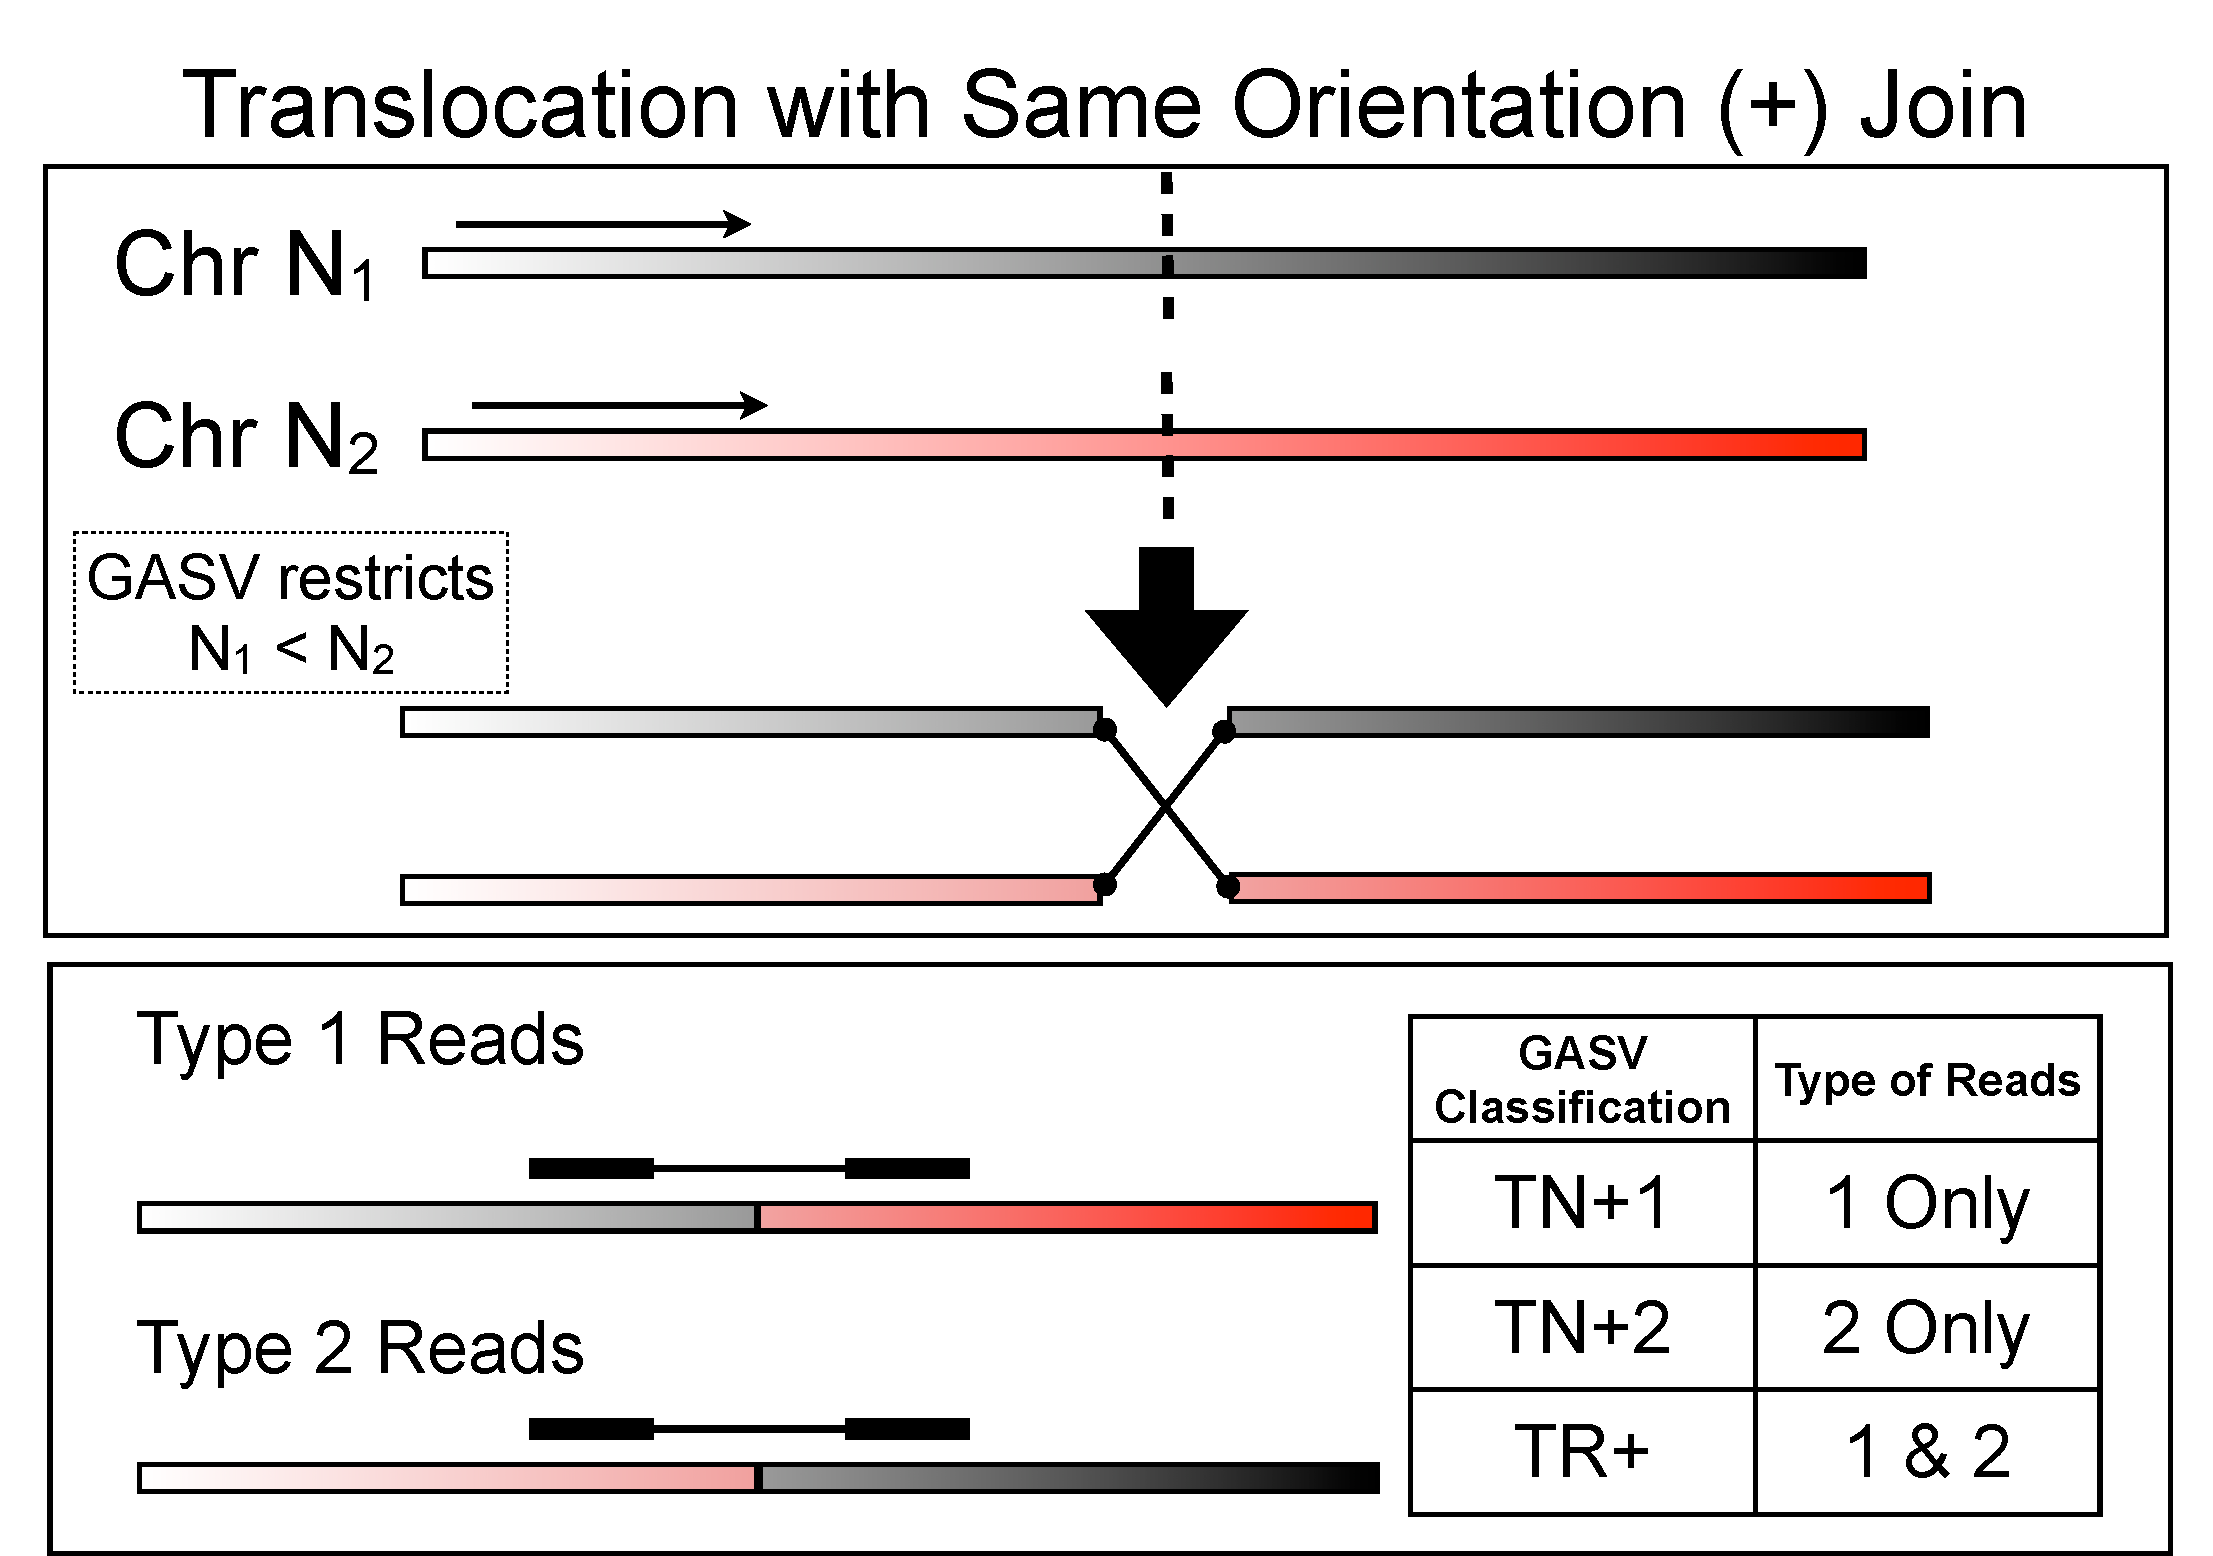
\includegraphics[width = 0.45 \textwidth] {Figures/Translocation_Same.pdf} % requires the graphicx package
  }
  \subfigure[Translocations: T-]{
   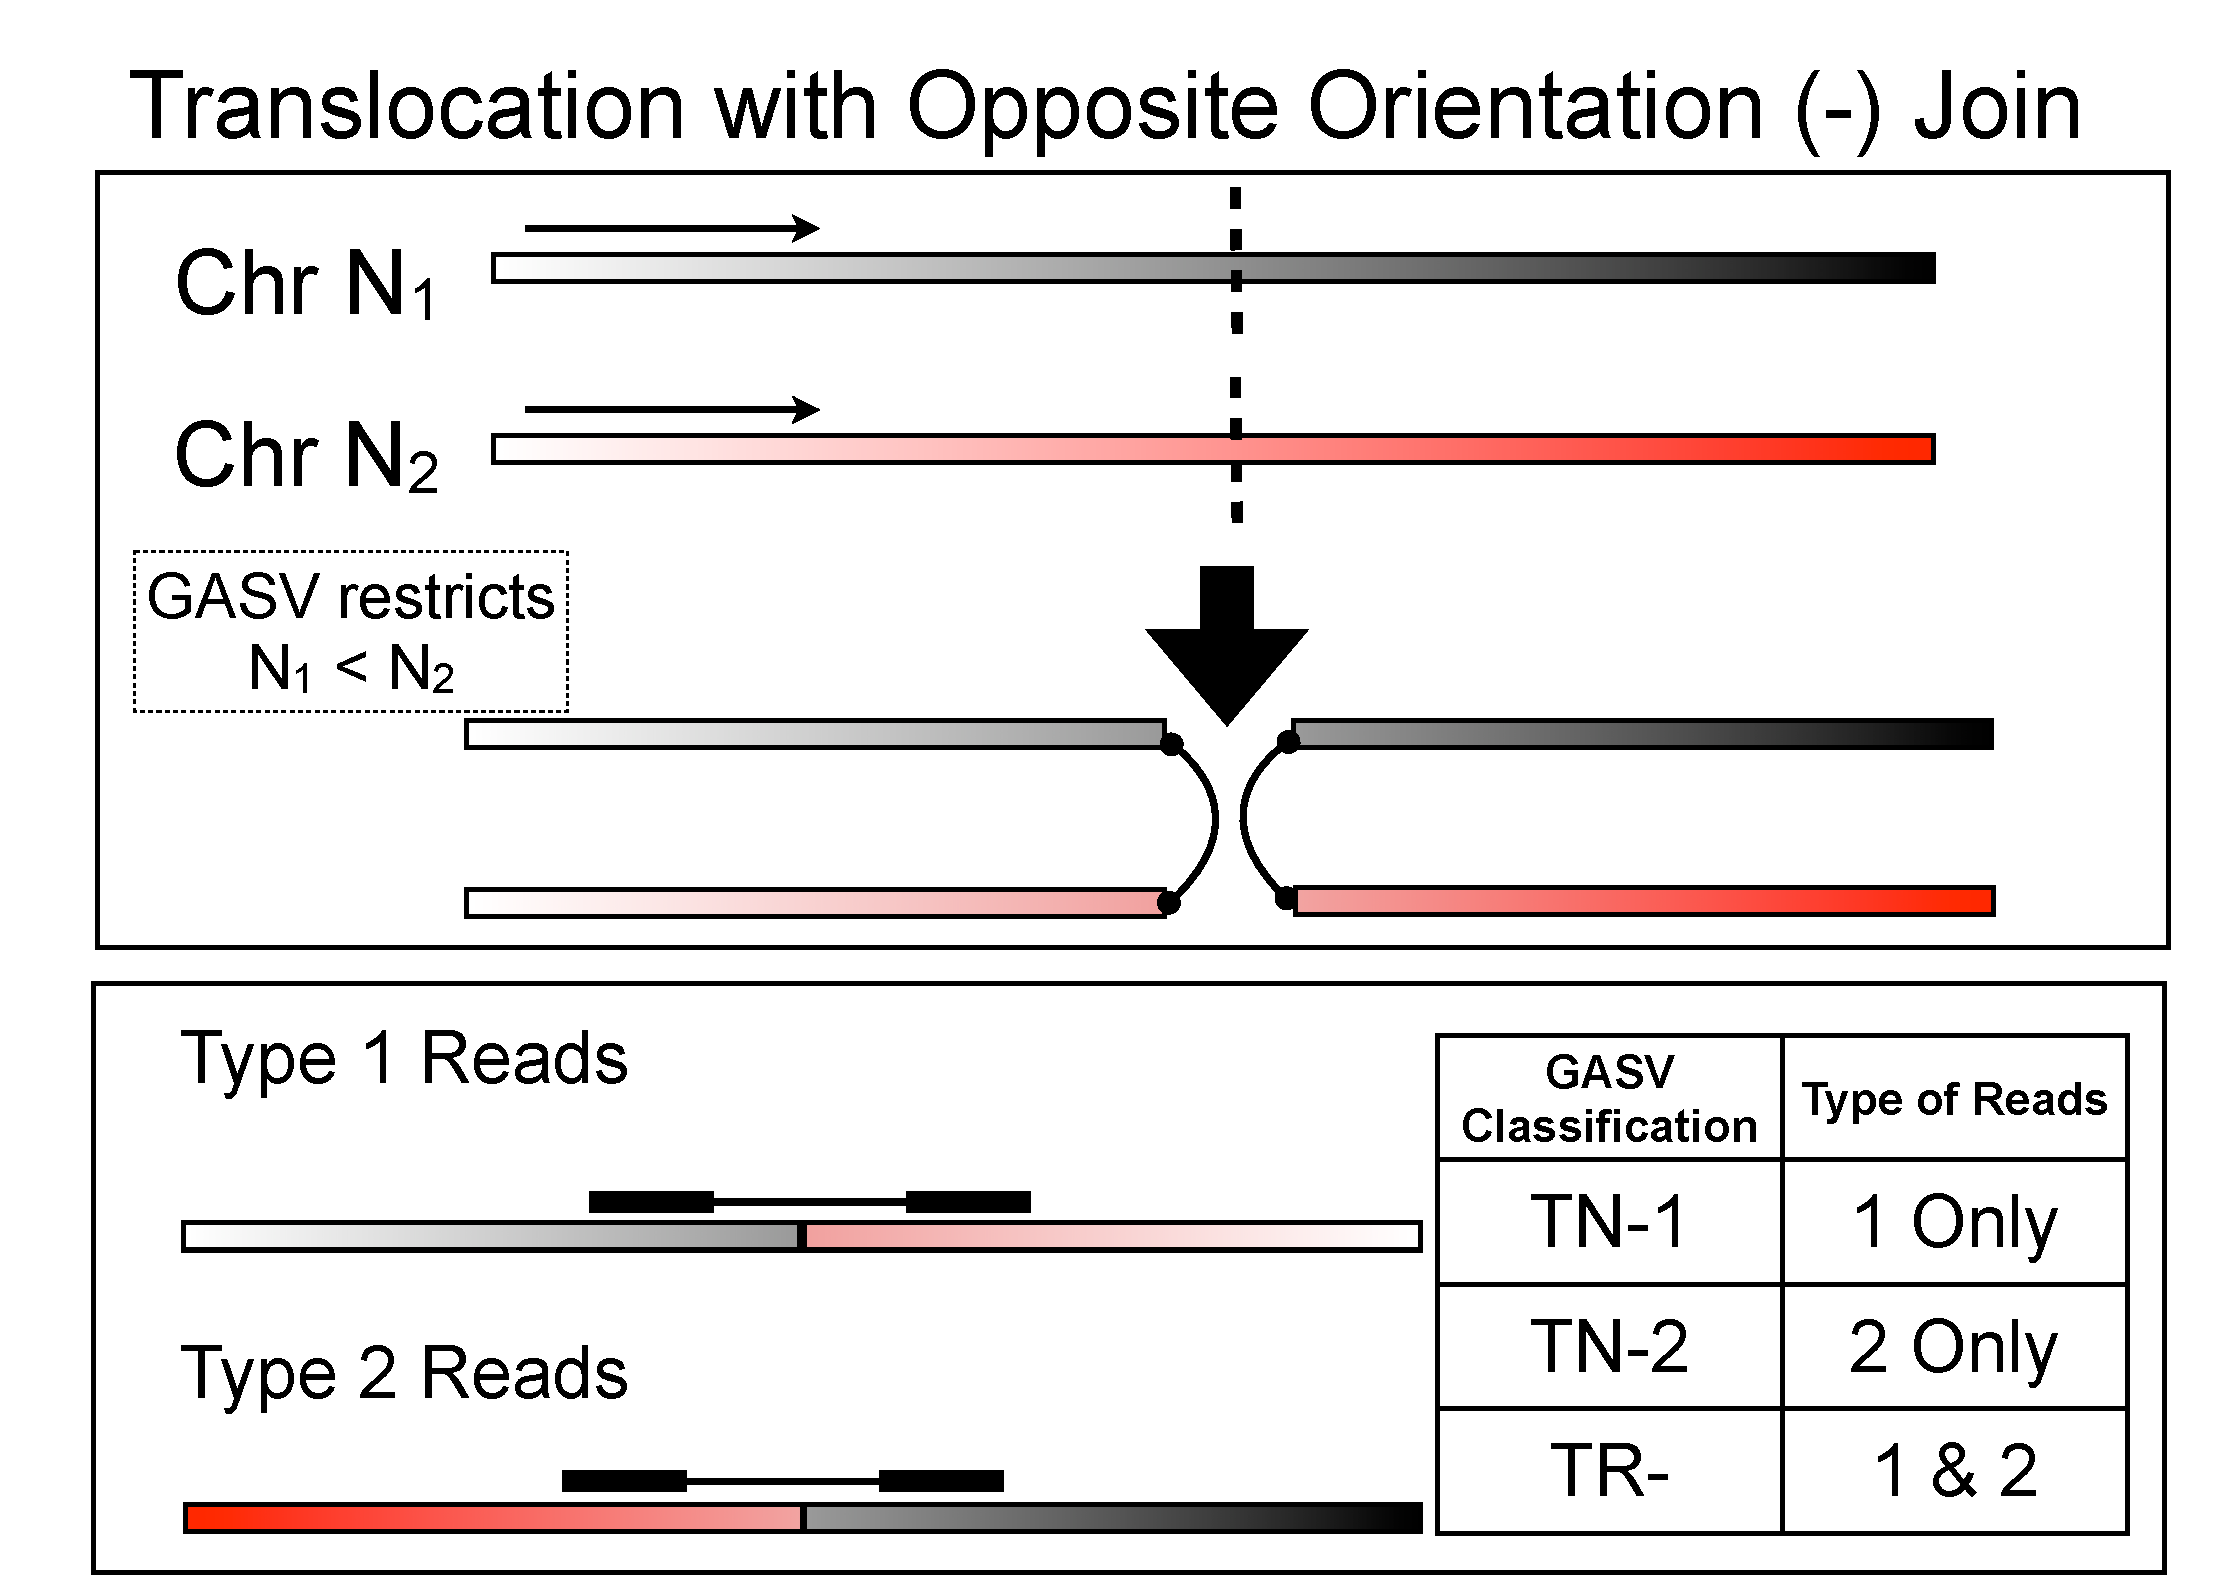
\includegraphics[width = 0.45 \textwidth] {Figures/Translocation_Opposite.pdf} % requires the graphicx package
   }
   \caption{\textbf{GASV Algorithm Translocation Definition.}}
   \label{fig:translocation}
\end{figure}

 \begin{wrapfigure}{l}{0.45 \textwidth}
    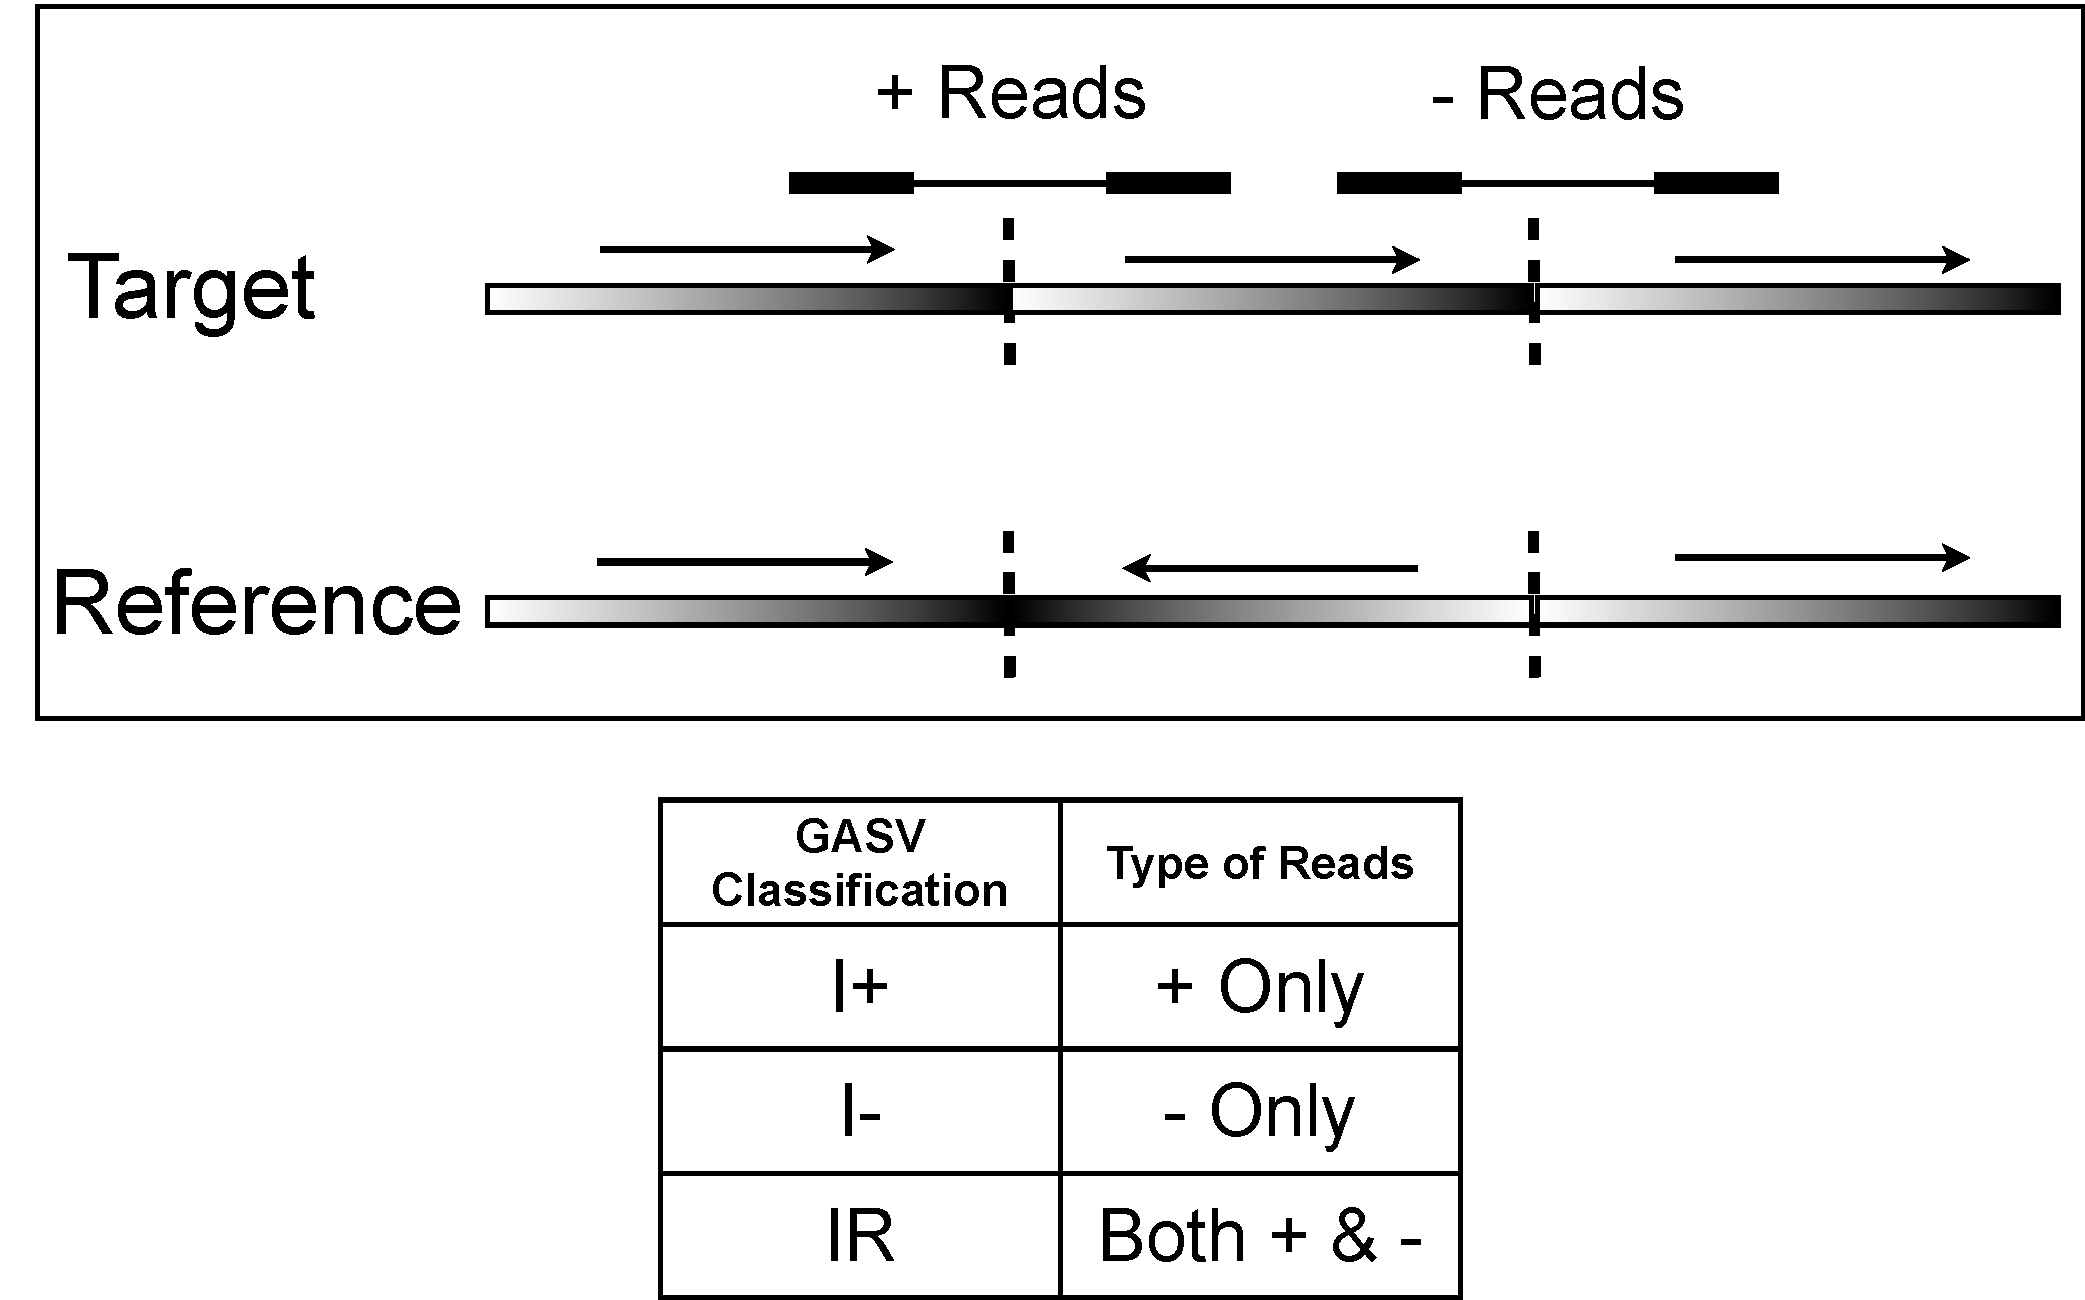
\includegraphics[width = 0.45 \textwidth] {Figures/Inversion.pdf} % requires the graphicx package
   \caption{\textbf{GASV Algorithm Inversion Definition.}}
   \label{fig:inversion}
\end{wrapfigure}

The GASV algorithm distinguishes between several types of translocations based on the orientations of the respective chromosomes at the join (Figure~\ref{fig:translocation}); opposite (-) or same (+); and which resulting chromosome in the test genome was observed; type 1 or type 2.  In the top panel of Figure~\ref{fig:translocation}, we illustrate the break and join event creating the translocation. While in the bottom panel, we show the resulting chromosomes present in the test genome, from which segments were sampled. As default mode, GASV will attempt to merge predictions from both type 1 and type 2 fragments to identify reciprocal translocation events (TR+ or TR-). If the -{}-noreciprocal flag has been set, clusters from type 1 and type 2 fragments will always be reported separately (TN-1, TN-2, TN+1, TN+2). A similar criteria applies to inversion structural variants (see Figure~\ref{fig:inversion}).

\subsubsection{Standard Clusters File Format}

Columns are tab-separated in the following format:

\begin{framed}
\begin{description}

\item[\#Cluster\_ID:]            Unique text identifier for the cluster
                         c$<$cluster\_number$>$. In -{}-maximal mode, the
                         sub-clusters are named as in:
                         c[MajorClusterNumber].[MinorSubclusterNumber]

\item[LeftChr:]                Chromosome containing the left breakpoint.

\item[LeftBreakPoint:]         Interval containing the left breakpoint.

\item[RightChr:]               Chromosome containing the right breakpoint.
			(Note that except for translocations LeftChr = RightChr).

\item[RightBreakPoint:]        Interval containing the right breakpoint.

\item[Num PRS:]                Number of PRs that support this variant.

\item[Localization:]           Square root of the breakpoint region (polygon of
                        intersection). The smaller the localization, the more
                        precisely the breakpoint can be determined. See below
                        for more information on localization.

\item[Type:]                   The type of structural variant indicated (See Section~\ref{sec:SVTypes}).
\end{description}
\end{framed}


\noindent Example Clusters File:


% Requires the booktabs if the memoir class is not being used
\begin{table}[htbp]\footnotesize
   \centering
   %\topcaption{Table captions are better up top} % requires the topcapt package
   \begin{tabular}{ llllllll } % Column formatting, @{} suppresses leading/trailing space
 \#Cluster\_ID:  &  LeftChr:   &  LeftBreakPoint: & RightChr:  &  RightBreakPoint:   &     Num PRS:  &  Localization:  &  Type: \\
		c521  &  17  &    40566182,40566330   &    17     &  40567335,40567463   &    4  &     86.4&    IR
    \end{tabular}
   \caption{GASV Default Clusters Format}
   \label{tab:booktabs}
\end{table}


\noindent \textbf{Note:} If the localization is equal to -1, this means that while a set
of PRs overlap, there is not a single structural variant that can
explain the data. Running GASV with the ``-{}-maximal'' flag will output
all maximal structural variant predictions from such a cluster.

For examples and more information on maximality, and localization
refer to Sindi, et al. (2009).

\subsubsection{Additional Output Options}
GASV provides two additional formatting options for the clusters file. These options are accessible by using the -{}-output $<$val$>$ option.

\begin{framed}
\begin{description}
\item[reads:]   The same as ``standard'' but has an additional column with a comma separated list of the names of names of PRs in each cluster. 

\item[regions:] Highly detailed output that specifying the coordinates
                         of the breakpoint polygon itself. The tab separated columns are:
                         \begin{itemize}
                         \item[] \#Cluster\_ID:	
                         \item[] Num PRS:
                         \item[] Localization:	
                         \item[] Type:	
                         \item[] List of PRS:	 
                         \item[]LeftChr:	
                         \item[] RightChr:
			\item[] Boundary Points:
			\end{itemize}
			The boundary points are given in the form: $x1, y1, x2, y2, \ldots$ where the points $(x_i,y_i)$ correspond to the boundary of the breakpoint polygon.
\end{description}
\end{framed}


\noindent Note: The output produced from GASV.jar may differ from output produced by earlier versions of GASV. Refer to RELEASE\_NOTES.txt for more information.
\clearpage

\section{GASVPro}

GASVPro is a probabilistic version of our original GASV algorithm.  GASVPro combines read depth information along with discordant paired-read mappings into a single probabilistic model. When multiple alignments of a read are given, GASVPro utilizes a Markov Chain Monte Carlo procedure to sample over the space of possible alignments.

\subsection{GASVPro Input Parameters}
Because GASVPro was designed to be run after BAMtoGASV and GASV, the input files to GASVPro will appear familiar to those who have experience with the GASV pipeline. There are also a number of probabilistic and statistical parameters that GASVPro requires.
\begin{description}
\item[] {\bf Input Files}{
\begin{description}
\item[] {\bf Clusters File}: must be in GASV Default Clusters Format (see section 4.3.2). {\bf NOTE:} The \verb+--output regions+ parameter must be passed to GASV to produce a clusters file of the correct format.
\item[] {{\bf Concordant File}: must be in BAMtoGASV default output format ($<$chr$>$ $<$start$>$ $<$end$>$). The BAMtoGASV preprocessor produces these files with the {\bf-WRITE\_CONCORDANT} option set to {\bf True}. See section 3.2 for details. {\bf This file {\em must} be sorted numerically by start coordinate.}}
\item[] {\bf Uniqueness Files}: must provide a directory in which uniqueness track files (of format $<$start$>$ $<$end$>$ $<$unique$>$) are named chr1\ldots chr$N$. {\bf These files also {\em must} be sorted numerically by start coordinate.}
\end{description}}



\item[] {\bf Numerical Parameters} {
\begin {description}
\item[] {\bf Average Fragment Length [Lavg] \& Average Read Length [ReadLen]}: {\em follow from sequencing libraries. In the event of multiple libraries, use the average over all datasets.}
\item[] {\bf Lambda \& Perr}: {\em parameters for probabilistic model, see manuscript.}
\item[] {\bf Minimum Fragment Size Limit}: this value is the smallest variant that GASVPro will use concordant coverage on.
\item[] {\bf Tolerance}: Tolerance is used to remove regions that have abnormally high
concordant coverage and, thus, can be eliminated from consideration
as a structural variant. A tolerance of $t$ will eliminate from further consideration as a potential structural variant a prediction with $N$ concordant fragments provided $P(\ge N$ $|$ no variant$) > t$.
\item[] {\bf Max Chromosome Number}: this is the highest {\em numerical value label} of all the chromosomes in the Clusters File.
\item[] {\bf Max Uniqueness Value}: this parameter is the value assigned to the most mappable regions in the uniqueness files. 
\item[] {\bf Minimum Scaled Uniqueness}: this parameter is the minimum value to which GASVPro will scale the uniqueness values for each variant. {\bf NOTE:} When this parameter is set to 1, all regions will have the same uniqueness value. 
\item[] {\bf Verbose}: specifying Y will print information for each cluster processed. 
\end{description}}
\end{description}
\subsection{Running GASVPro}

There are two ways to run GASVPro: via command-line arguments or via a parameters file. We have provided a parameters file for running GASVPro, and highly recommend its use for convenience and to ensure input accuracy. The parameters file also allows for clean record-keeping and can be annotated.
\begin{figure}[H]
\begin{Verbatim}[frame=single]
# A Sample GASVPro parameters file
# Annotation can appear on any line beginning with a hash mark (#).
clusterFile: <ClusterFile>
ConcordantFile: <ConcordanceFile>
UNIQUEFile: <UniquenessFile/Directory>
Lavg: <value>
ReadLen: <value>
Lambda: <value>
Perr: <value>
Limit: <value>
Tolerance: <value>
MaxChrNumber: <value>
MaxUniqueValue: <value>
MinScaledUniqueness: <value>
Verbose: Y
\end{Verbatim}
\caption{\bf A Sample GASVPro Parameters File}
\end{figure}
\noindent Using a parameters file allows the user to run GASVPro with the following command:
	\begin{Verbatim}[frame=single]
% ./GASVPro {ParametersFile}
	\end{Verbatim}
%\noindent Alternatively, it is possible to run GASVPro using only command line arguments, as follows. This method is not preferred, however, as it can easily lead to input errors. 
%\begin{Verbatim}[frame=single]
%% ./GASVPro {ClusterFile} {ConcordanceFile} {UniquenessFile/Directory} {Lavg} 
%{ReadLen} {Lambda} {Perr} {Limit} {Tolerance} {MaxChrNumber} { MaxUniqueValue} 
%{MinScaledUniqueness} {Verbose}
%\end{Verbatim}

\subsection{GASVPro Output}
After successful completion GASVPro will output two files, a \verb+.clusters+ file and a \verb+.coverage+ file. Input parameters relevant to subsequent steps in the GASV pipeline will also be included in the filenames. The \verb+.clusters+ file contains the variance probabilities that GASVPro calculated. Here is an example GASVPro output, contained in the \verb+.clusters+ file:
\begin{table}[htbp]\footnotesize
   \centering
   %\topcaption{Table captions are better up top} % requires the topcapt package
   \begin{tabular}{llllllll} % Column formatting, @{} suppresses leading/trailing space
 \#Cluster\_ID \& Variance:  &  NumPRS:   &  Localization: & Type:  &  List of PRS:   &     $\cdots$  & $\cdots$  &  $\cdots$ \\
		\verb+c521_-650.01_-297.342+  &  \verb+1+  &    \verb+189+   &    \verb+D+     &  \verb+chr17_41883_42105_0:0:0_2:0:0_15789d3+   &    $\cdots$  &     $\cdots$&    $\cdots$
    \end{tabular}
   \caption{An Example GASVPro Output Cluster}
   \label{tab:booktabs}
\end{table}

\noindent The field \verb+c1_-650.01_-297.342+ has the cluster name `c1' appended with 
the likelihood c1 is a variant (\verb+-650.01+) and the likelihood that c1
is not a variant (\verb+-297.342+). The rest of the information in the \verb+.clusters+ file is carried over from the input file. 


\end{document}  
